% Redrawn from https://gregable.com/2008/11/i/pq-tree.webp
% Rebuild: latex -interaction=nonstopmode -halt-on-error pq-tree-1.tex
%          dvisvgm --no-fonts --exact-bbox --bbox=papersize pq-tree-1.dvi -o pq-tree-1.svg
\documentclass[tikz,border=4pt]{standalone}
\usetikzlibrary{backgrounds}
\pgfdeclarelayer{edges}
\pgfsetlayers{background,edges,main}
\begin{document}
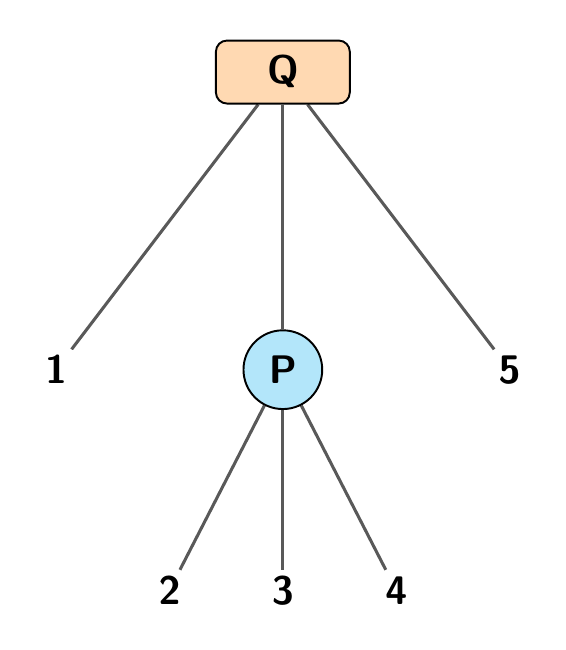
\begin{tikzpicture}[x=12mm,y=14mm,line width=.7pt,
  background rectangle/.style={fill=white},show background rectangle,
  every node/.style={font=\sffamily\bfseries\Large},
  edge/.style={draw=black!65,line width=1.1pt},
  leaf/.style={fill=white,inner sep=2pt}]
\node[draw,rounded corners=4pt,fill=orange!30,minimum width=17mm,minimum height=8mm] (q) at (2.4,4.7) {Q};
\node[circle,draw,fill=cyan!30,minimum size=10mm,inner sep=0pt] (p) at (2.4,2) {P};
\node[leaf] (l1) at (0,2) {1};
\node[leaf] (l2) at (1.2,0) {2};
\node[leaf] (l3) at (2.4,0) {3};
\node[leaf] (l4) at (3.6,0) {4};
\node[leaf] (l5) at (4.8,2) {5};
\begin{pgfonlayer}{edges}
  \foreach \child in {l1,p,l5} \draw[edge] (q) -- (\child);
  \foreach \child in {l2,l3,l4} \draw[edge] (p) -- (\child);
\end{pgfonlayer}
\end{tikzpicture}
\end{document}
